\documentclass[a4paper,12pt]{article}
\usepackage[utf8]{inputenc}
\usepackage[english]{babel}
\usepackage{subfigure}
\usepackage{graphicx}

% Title Page
\title{Upper limit for High mass X$\rightarrow$WW search}
\author{Piergiulio Lenzi}


\begin{document}
\maketitle

\begin{abstract}
\end{abstract}

\section{Introduction}
In this report we will study the statistical approach to the upper limit computation for a high energy physics search for a new particle.
We will use data from the 2015 run of the CMS experiment at the LHC and the corresponding Monte Carlo (MC) simulations.

We will search for a new signal in the $WW\rightarrow{}2l2\nu$ final state. This channel is also a decay channel for the Standard Model Higgs boson (H). 
We will however search for an additional particle, named X in the following, that is supposed to be heavier than H. 
We will scan a wide range of masses for X and, if we do not find a compelling evidence for a signal, we will set an upper limit on the  cross section of X.

\section{The physics case}
In this experience we will search for the existence of a new hypothetical high mass particle, named X. {\bf We expect this particle to be a heavy variant of the Standard Model Higgs boson}. 
For this reason we hypothesize that X shares with H the production mechanism. This is a reasonable assumption that is verified in several new physics models.
In particular we assumes that X can be produced via two main production mechanisms, called gluon fusion (ggF) and vector boson fusion (VBF), represented by the diagrams in Fig.~\ref{fig:prod}.
\begin{figure}
 \centering
 \subfigure[ggF]{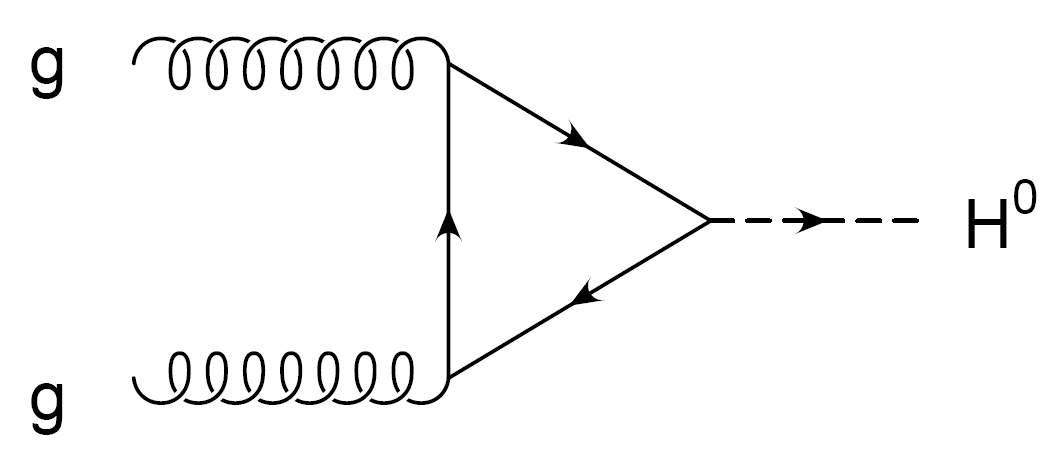
\includegraphics[width=0.4\textwidth]{images/gluon_fusion.png}}
 \subfigure[VBF]{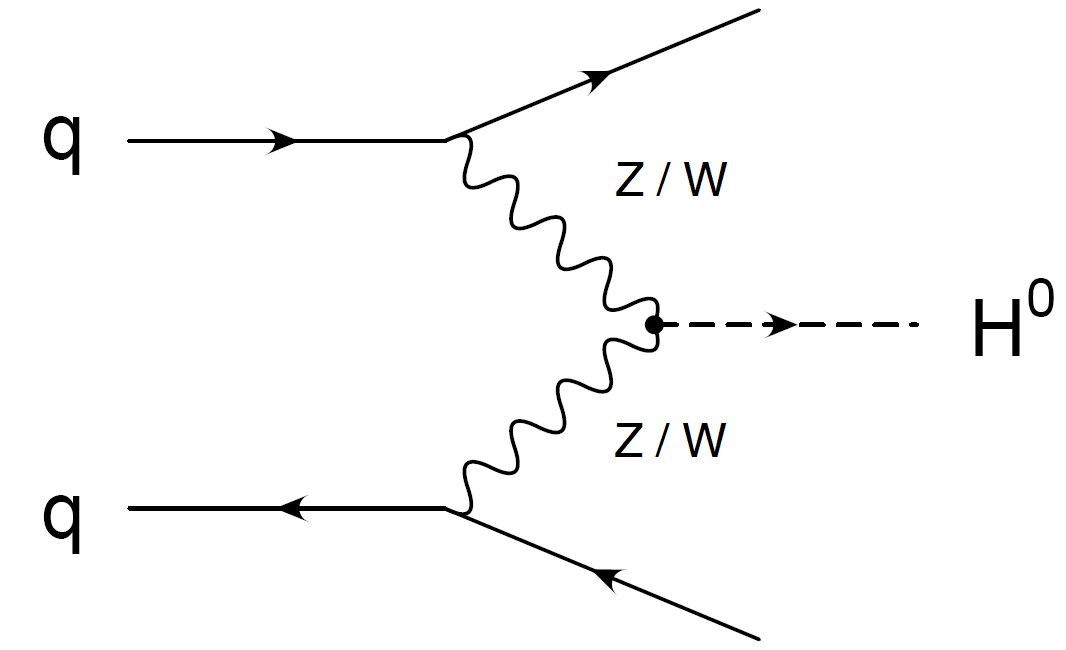
\includegraphics[width=0.3\textwidth]{images/vector_boson_fusion.png}}
 \caption{Feynmann diagrams of the two main production mechanisms for X.\label{fig:prod}}
\end{figure}

The details and precise meaning of the Feynman dagrams of Fig.~\ref{fig:prod} are not relevant for this exercise, the relevant piece of information is that two mechanisms are available and that 
they are marked by a substantial difference: {\bf the ggF shows no other particles in the final state beyond X, the VBF has two quarks in addition to the X in the final state}.
Although it should be noted that a precise calculation shows that additianal particles in the form of hadronic jets can also arise in ggF, it remains true that events arising from the two mechanisms 
are different when it comes to the number of jets produced in addition to the X particle.

The production cross section for the Higgs boson as a function of its mass is reported in Fig.~\ref{fig:production}. Although we now know the mass of the Higgs boson to be 125 GeV, this plot is useful
because it can be used as a model for the expected cross section for X.
\begin{figure}
 \centering 
 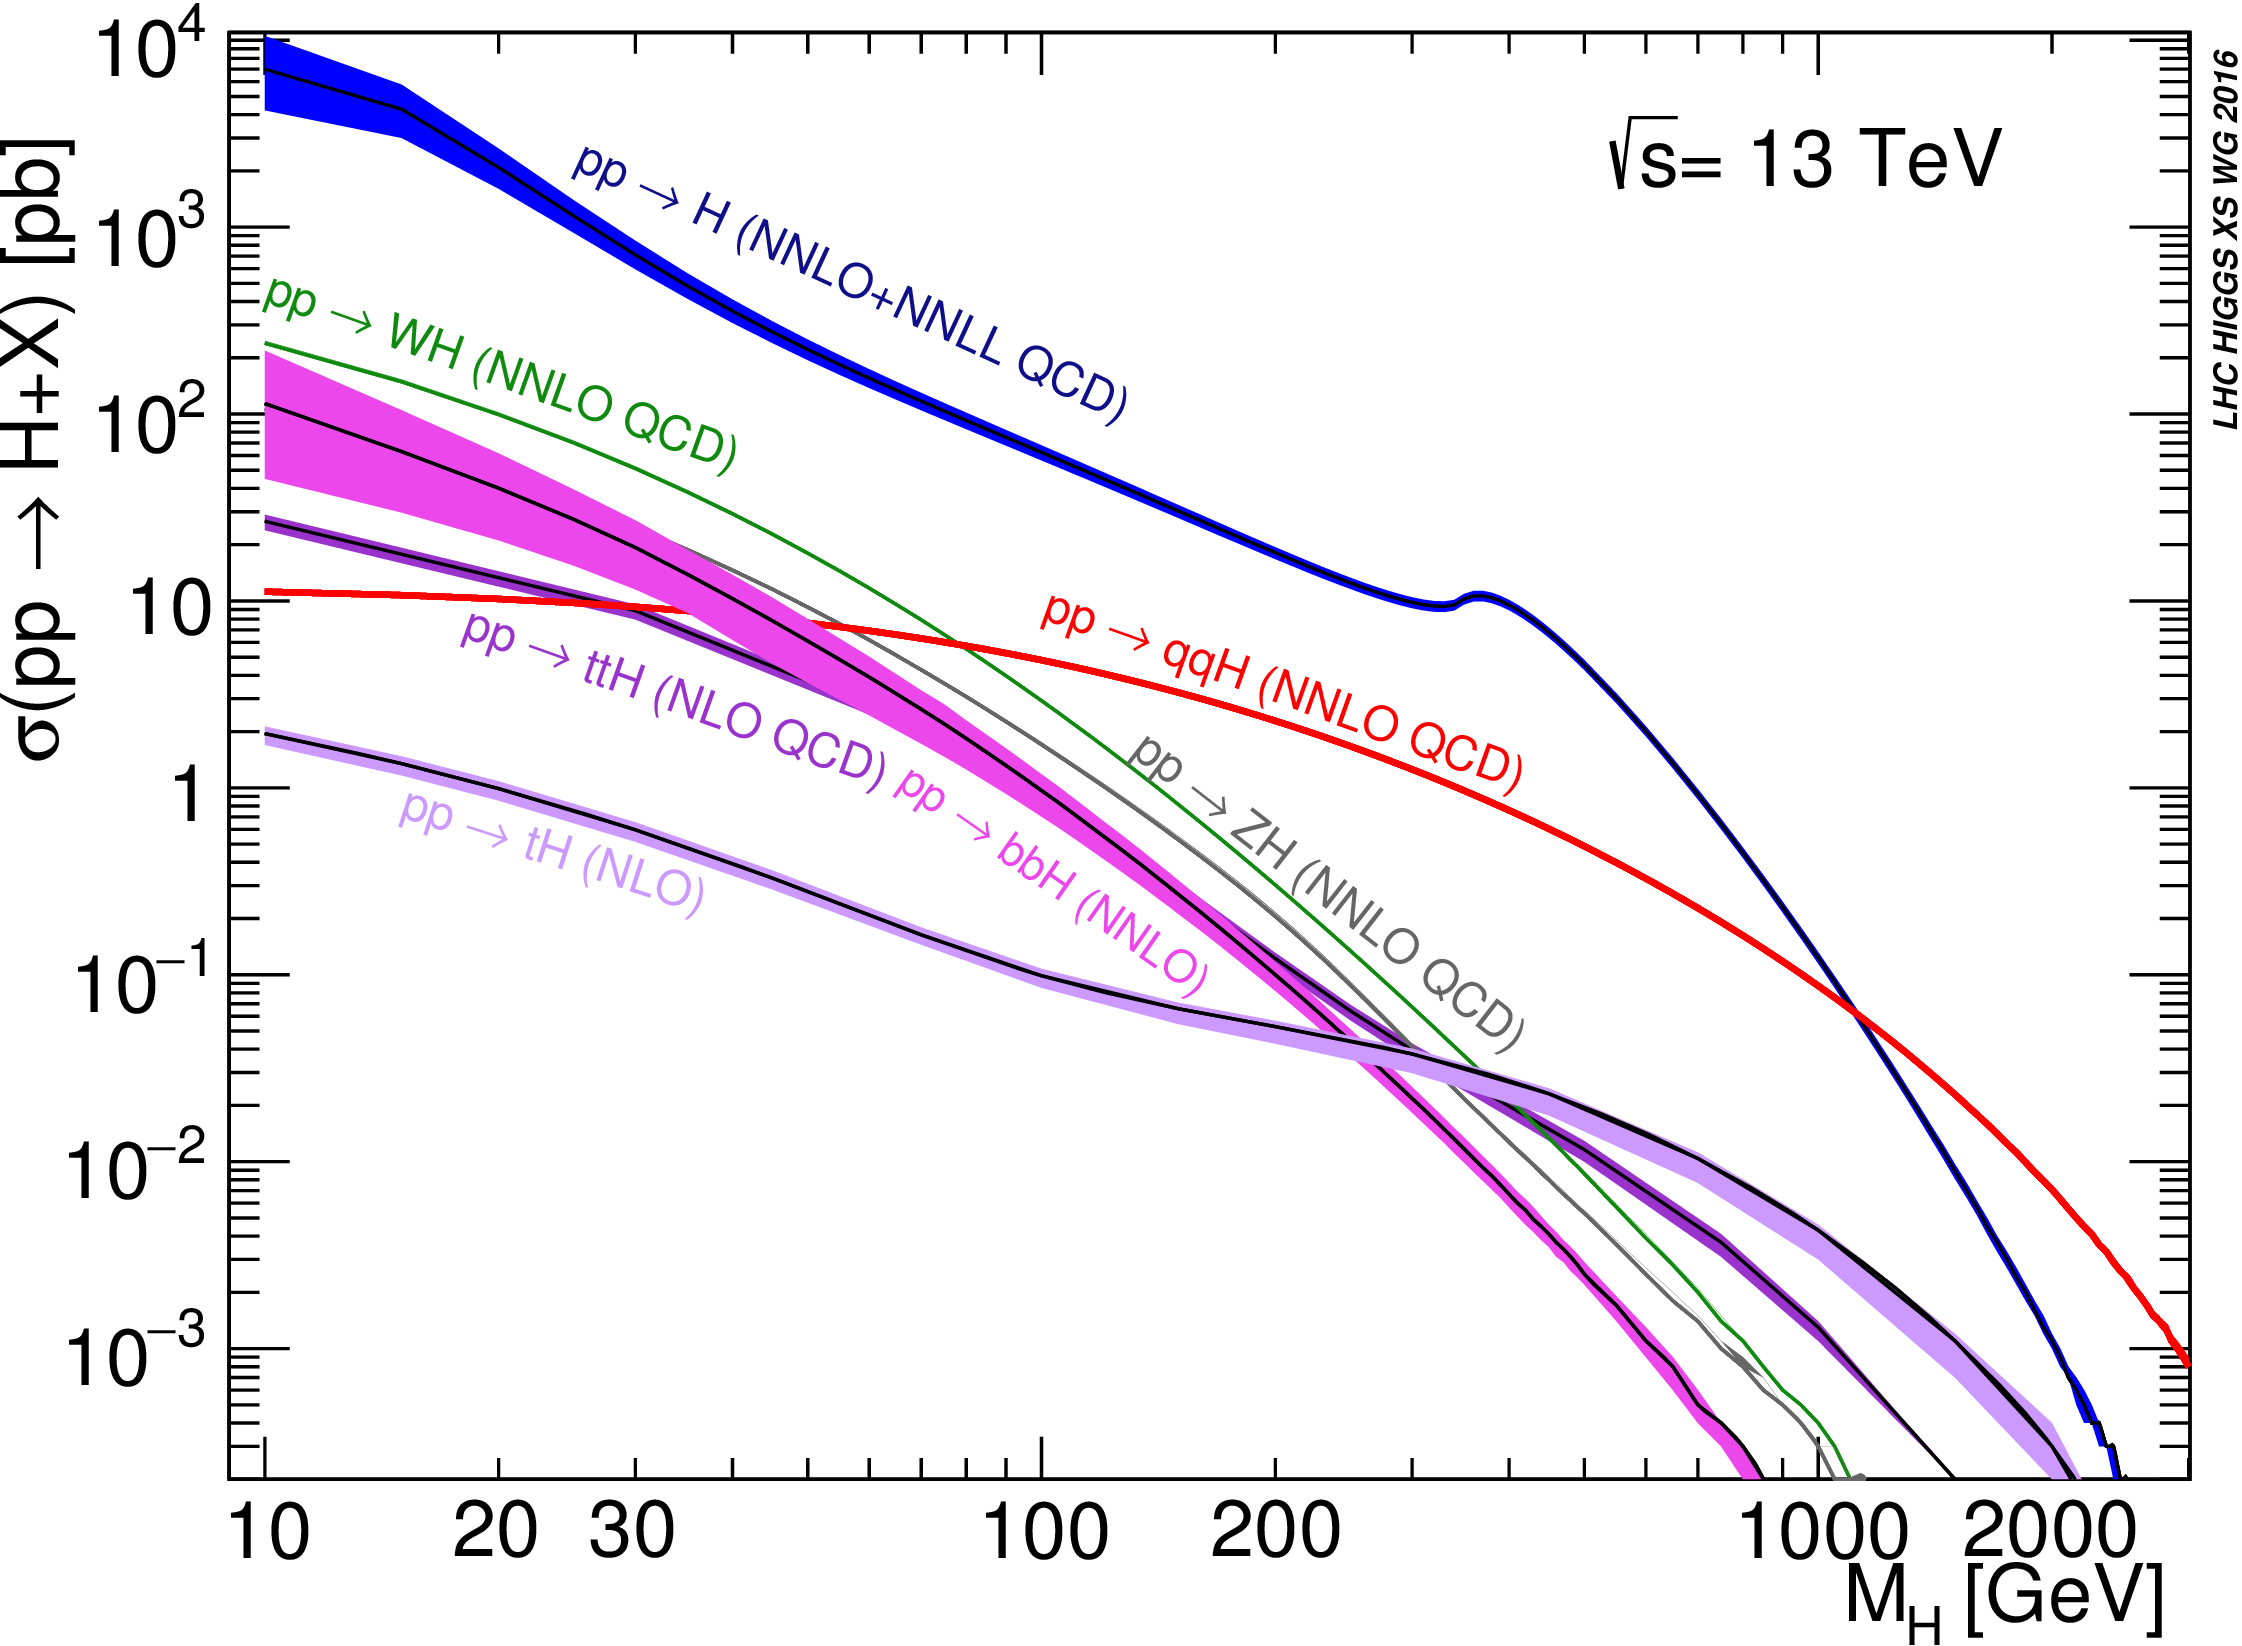
\includegraphics[width=0.5\textwidth]{images/plotAll_13tev_BSM_sqrt.png}
 \caption{Standard model Higgs boson cross section as a function of the mass of the Higgs boson. The ggF mechanisms is labeled $pp\rightarrow{}H$, the VBF mechanism is labeled $pp\rightarrow{}qqH$. Also other, sub-leading mechanisms are reported, 
 which we will neglect.\label{fig:production}}
\end{figure}

We will assume that the cross section $\sigma$ for each of the production channels of X scales with a common factor $\mu$ of the corresponding Higgs boson cross section:
\begin{equation}
 \sigma_{X [ggF,VBF]}(M) = \mu(M)\sigma_{H [ggF,VBF]}(M)
\end{equation}
 where M is the mass of X, and obvious meaning of the other symbols. This is a reasonable assumption, verified by several new physics models.
We notice that {\bf the relative importance of the VBF mechansm grows with the X mass}, and becomes dominant above \~1.5 TeV.
 
 We will assume that, like H, also X has several decay channels. X in particular has the same branching ratios of H, which are summarized in Fig.~\ref{fig:br}.
\begin{figure}
 \centering 
 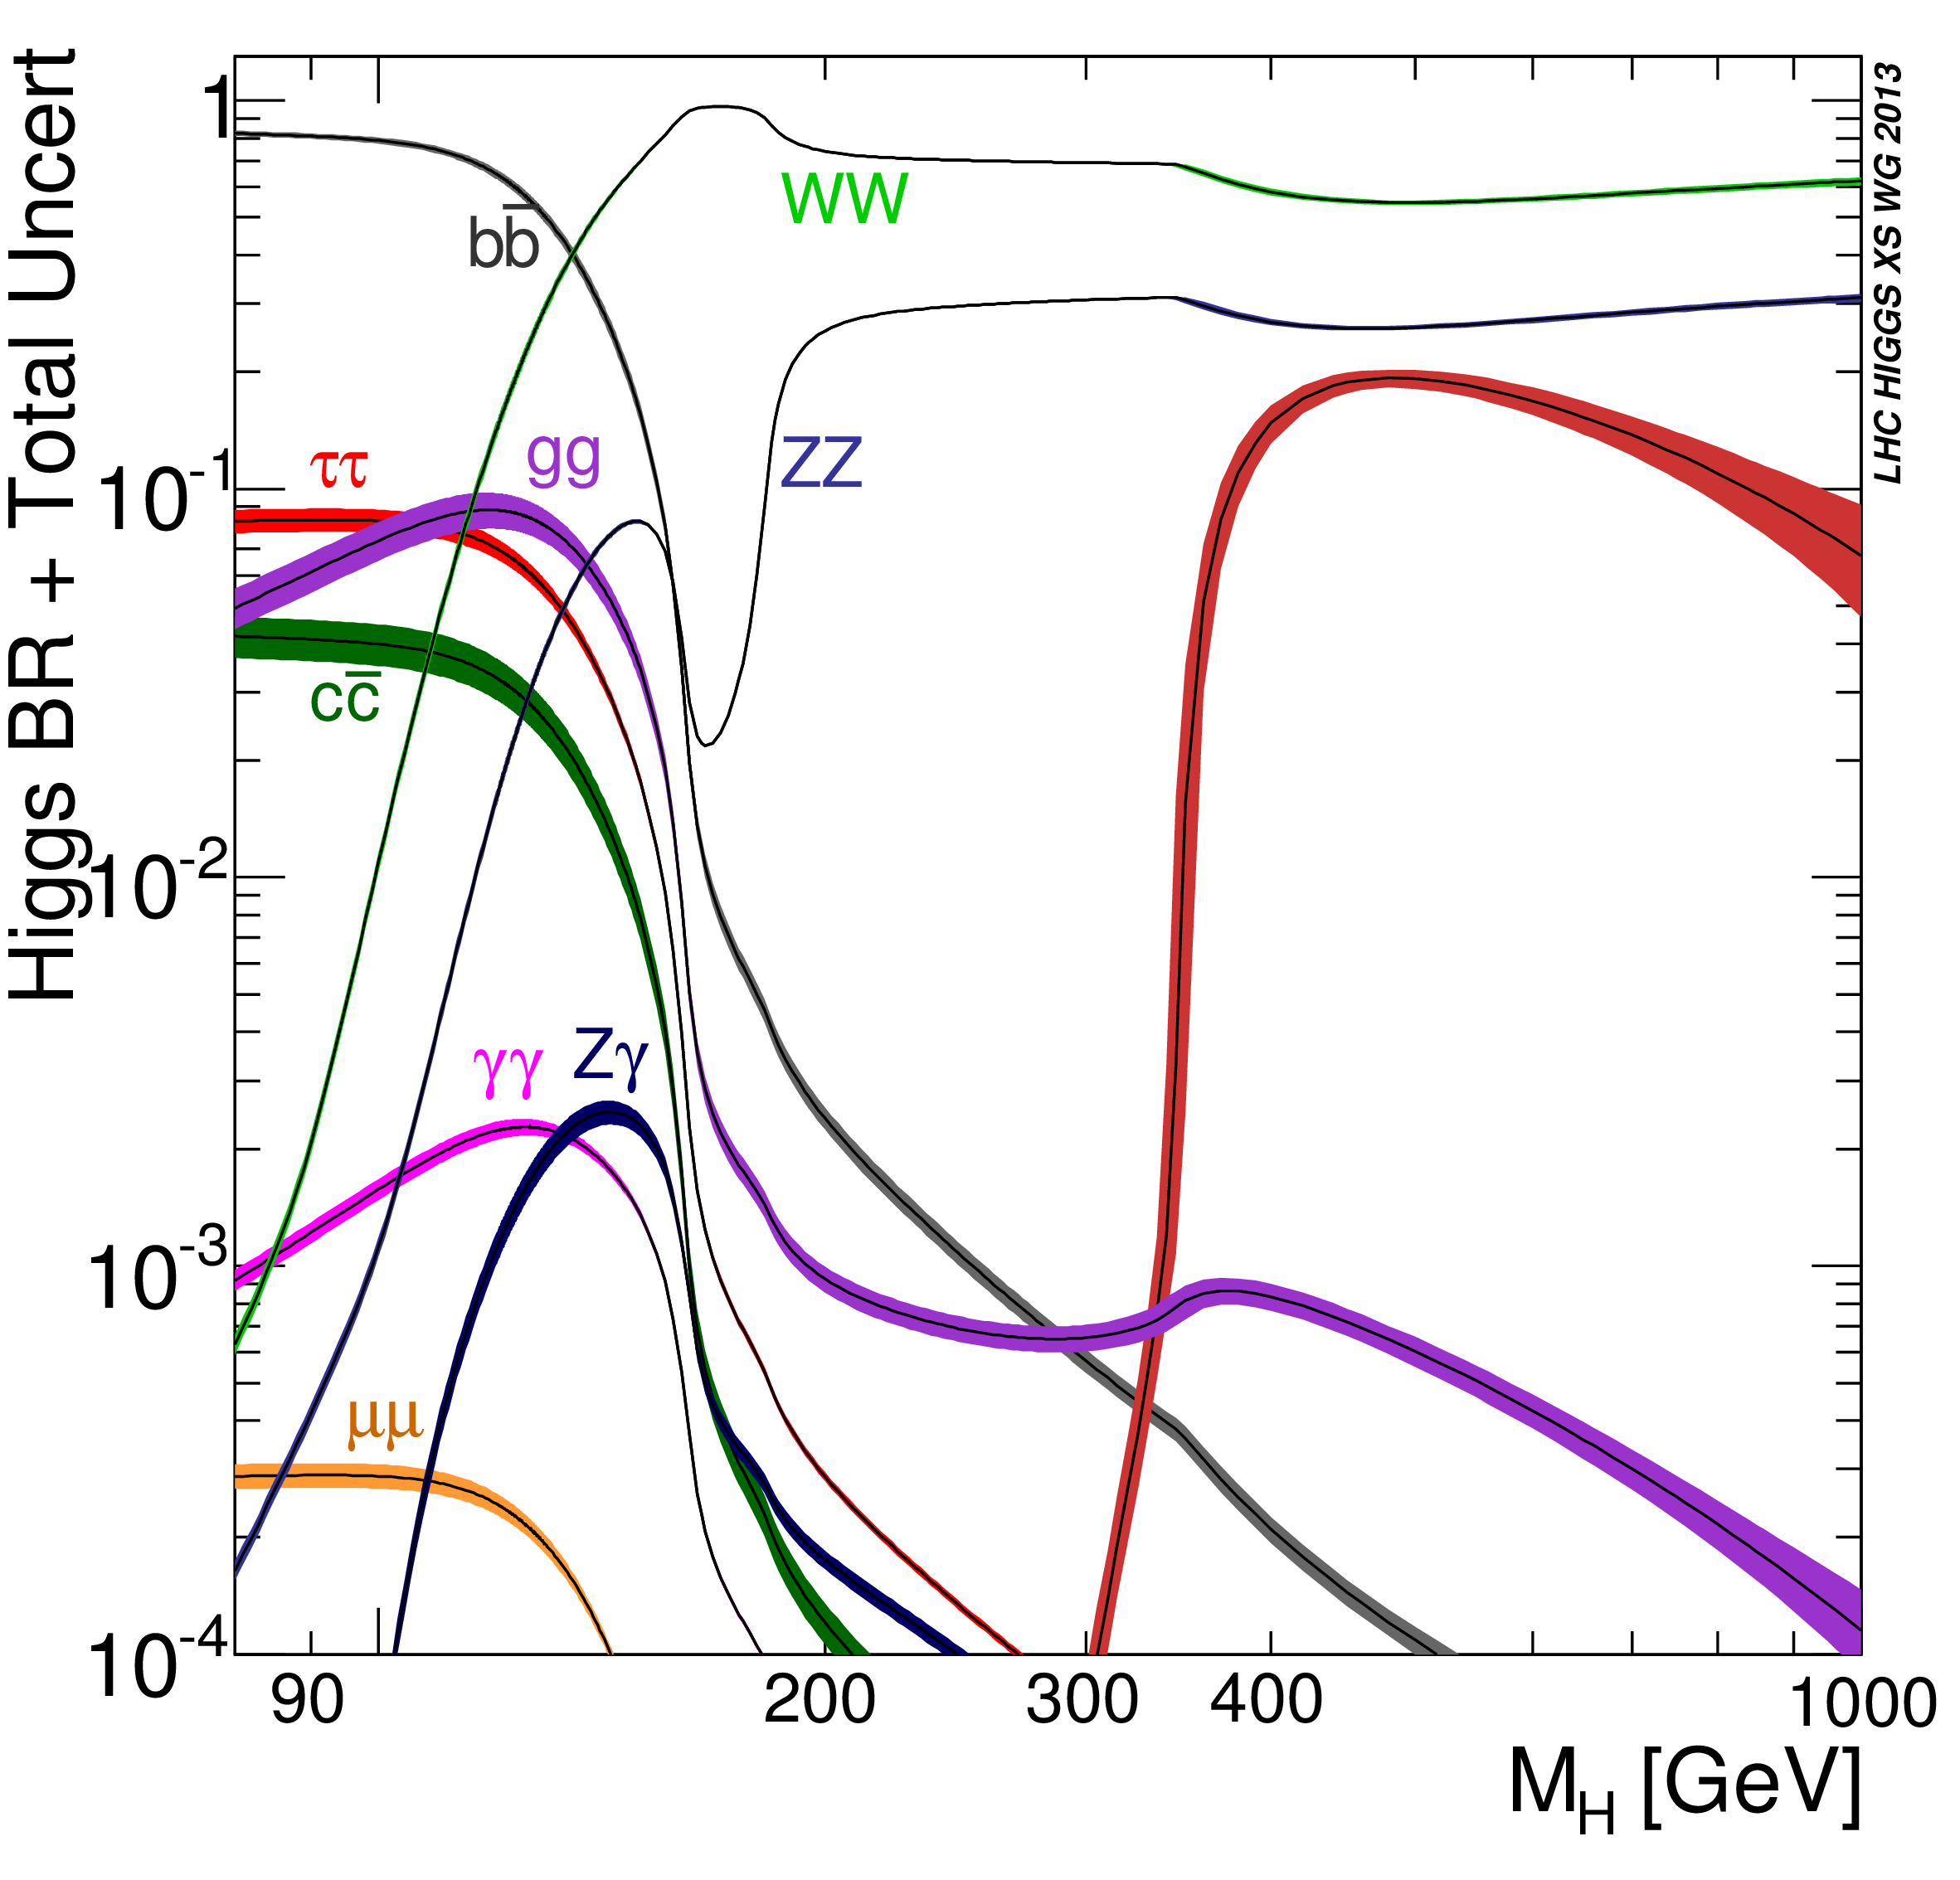
\includegraphics[width=0.5\textwidth]{images/Higgs_BR.png}
 \caption{Standard model Higgs boson cross section as a function of the mass of the Higgs boson. The ggF mechanisms is labeled $pp\rightarrow{}H$, the VBF mechanism is labeled $pp\rightarrow{}qqH$. Also other, sub-leading mechanisms are reported, 
 which we will neglect.\label{fig:br}}
\end{figure}






\end{document}          
